\documentclass[10pt]{article}
\usepackage{icmlko}

\icmlmeta{IP 파운데이션 월드모델}{185}{트리의 우위는 긁어온 열에서만 산다}{노트 155부터 여덟 노트가 ``선형이 더 나은 지렛대인데 판은 트리를 뽑는다''를 되풀이했다. 열을 갈라 보니 둘이 같은 열에서 안 싸우고 있었다}

\begin{document}

\twocolumn[
\icmlheader

\begin{abstract}
노트 184가 ``F18 배깅이 아홉 도메인 중 여덟에서 F6 능형을 이기는데 지는
하나가 팝업''을 남기고 ``팝업 축 다섯이 사람이 읽어 매긴 것이라 그런가''를
걸었다. \textbf{그 가설은 아니다} --- 공유 축 다섯으로만 제한하면 팝업의
격차가 $-$0.070 에서 $-$0.013 으로 오히려 \emph{줄고}, 애초에 그 다섯은
팝업에서만 사람이 매긴 것이고 나머지 아홉은 긁어온 값을 다섯 칸에 넣은
것이다(노트 164). \textbf{대신 훨씬 큰 것이 나왔다.} 열을 출처로 갈랐다 ---
공유 축 다섯 대 긁어온 축(검색 · 달력 · 위키). \textbf{트리의 우위 전부가
긁어온 열에서 나온다.} 판 격차가 전체 축에서 $+$0.0775($t{=}5.95$),
\textbf{공유 다섯만에서 $+$0.0122($t{=}0.78$ --- 안 갈린다)}, 긁어온
축만에서 $+$0.0931($t{=}6.14$)이다. 이기는 도메인도 8/9 $\to$ \textbf{5/9}
$\to$ 8/9 로 같이 움직인다. 게임이 극단이다 --- 공유 다섯에서 능형이
\textbf{$+$0.262} 앞서고 긁어온 축에서 배깅이 $+$0.155 앞선다. 같은
도메인이 열 출처에 따라 양쪽 끝을 다 간다. \textbf{이걸로 여덟 노트짜리
긴장이 풀린다.} 노트 155$\sim$172 가 ``선형이 더 나은 지렛대''를 여섯 번
확인했고 노트 184 가 ``판은 트리를 뽑는다''를 확인했는데, \textbf{둘이 같은
열에서 안 싸우고 있었다} --- 판의 트리 선호는 \emph{지렛대가 아닌} 열에서
온다. 그래서 실무 결론이 하나 떨어진다: \textbf{조언용 모형으로 능형을
써도 공유 축에서는 판을 거의 안 잃는다}($+$0.0122 · 안 갈림). 지금까지
``판을 올리려면 트리, 조언하려면 선형''이라는 맞바꿈으로 읽었는데
\textbf{맞바꿈이 아니었다.}
\end{abstract}
]

\begin{figure*}[t]
\centering
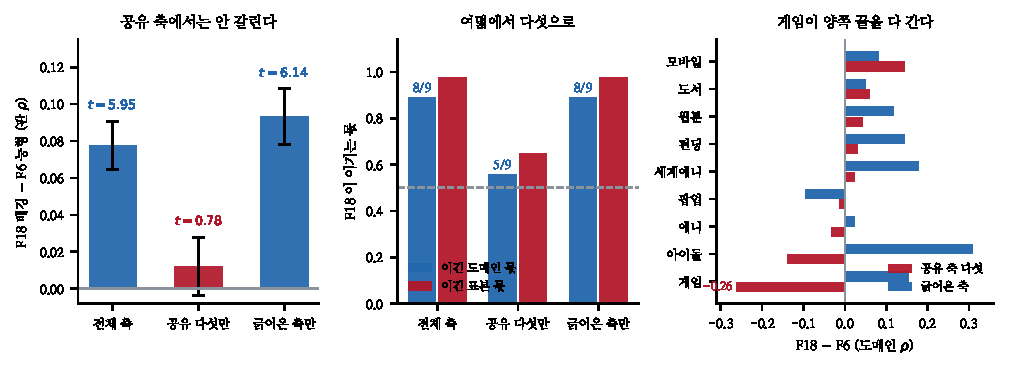
\includegraphics[width=\textwidth]{figs/prov.pdf}
\caption{왼쪽 --- 공유 축에서는 안 갈린다. 가운데 --- 여덟에서 다섯으로.
오른쪽 --- 게임이 양쪽 끝을 다 간다.}
\end{figure*}

\section{걸었던 가설은 아니다}

\claimx{\textbf{팝업의 격차가 오히려 준다} --- 전체 축에서 $-$0.070 인데
공유 다섯만 쓰면 $-$0.013 이다. ``사람이 매긴 축이라 선형이 낫다''면
반대로 커져야 한다.}{그리고 전제 자체가 틀렸다 --- 공유 축 다섯은
\emph{팝업에서만} 사람이 매긴 것이고 나머지 아홉은 긁어온 값을 그 칸에
넣은 것이다(노트 164 · \texttt{docs/AXIS\_MEANING.md}). 게임의
\texttt{goods\_scale} 은 디스크 용량 GB 다.}

\section{열을 출처로 갈랐다}

\begin{table}[t]
\centering\tsize
\caption{F18 배깅 $-$ F6 능형. 짝 부트스트랩 400회.}
\begin{tabular}{lrrl}
\toprule
열 집합 & 차 & sd & \\
\midrule
전체 축 & $+$.0775 & .0130 & $t{=}5.95$ \\
\textbf{공유 축 다섯만} & \textbf{$+$.0122} & .0157 & \textbf{$t{=}0.78$} \\
긁어온 축만 & $+$.0931 & .0152 & $t{=}6.14$ \\
\bottomrule
\end{tabular}
\end{table}

\begin{table}[t]
\centering\tsize
\caption{F18 이 이기는 도메인.}
\begin{tabular}{lrr}
\toprule
& 도메인 & 표본 몫 \\
\midrule
전체 축 & 8/9 & 97.7\% \\
\textbf{공유 축 다섯만} & \textbf{5/9} & \textbf{65.0\%} \\
긁어온 축만 & 8/9 & 97.7\% \\
\bottomrule
\end{tabular}
\end{table}

\claimx{\textbf{공유 축에서는 트리와 선형이 안 갈린다}($t{=}0.78$ · 트리가
이길 붓스트랩 확률 80\%). 긁어온 축에서는 $t{=}6.14$ 로 확실히
갈린다.}{\textbf{긁어온 축만 쓴 격차가 전체 축보다 크다}($+$0.0931 대
$+$0.0775) --- 공유 축을 섞으면 트리의 우위가 희석된다. 즉 공유 축은
트리에게 도움이 안 될 뿐 아니라 살짝 방해가 된다.}

\begin{table}[t]
\centering\tsize
\caption{도메인별 F18 $-$ F6.}
\begin{tabular}{lrrr}
\toprule
& 공유 다섯 & 긁어온 & 전체 \\
\midrule
\textbf{게임} & \textbf{$-$.262} & \textbf{$+$.155} & $+$.036 \\
아이돌 & $-$.138 & $+$.308 & $+$.160 \\
애니 & $-$.032 & $+$.024 & $+$.028 \\
팝업 & $-$.013 & $-$.095 & $-$.070 \\
\midrule
모바일 & $+$.144 & $+$.082 & $+$.146 \\
웹툰 & $+$.042 & $+$.118 & $+$.108 \\
\bottomrule
\end{tabular}
\end{table}

\claimx{\textbf{게임이 양쪽 끝을 다 간다} --- 공유 다섯에서 능형이 0.262
앞서고 긁어온 축에서 배깅이 0.155 앞선다. \emph{같은 도메인 · 같은
레코드}인데 어느 열을 주느냐로 승자가 바뀐다.}{게임 공유 축은 스팀
메타(장르 수 · 퍼블리셔 · 가격 · 디스크 용량)이고 긁어온 축은 위키 조회수
· 검색 · 달력이다. \textbf{앞쪽은 매끈하고 뒤쪽은 덩어리져 있다} --- 트리는
덩어리를 쪼개서 먹고 선형은 매끈한 것을 곧게 편다.}

\section{여덟 노트짜리 긴장이 풀린다}

\begin{table}[t]
\centering\tsize
\caption{이 흐름이 되풀이한 두 관찰.}
\begin{tabular}{ll}
\toprule
노트 155$\sim$172 & 선형이 더 나은 지렛대다 (여섯 번) \\
노트 156 · 161 · 171 · 174 · 184 & 판은 트리를 뽑는다 \\
\midrule
\textbf{노트 185} & \textbf{둘이 같은 열에서 안 싸운다} \\
\bottomrule
\end{tabular}
\end{table}

\claimx{\textbf{판의 트리 선호는 지렛대가 아닌 열에서 온다.} 지렛대가 될
수 있는 것은 공유 축 다섯뿐인데(노트 172: 타깃 폭과 굿즈 규모는 조언할 수
있다) 거기서는 트리와 선형이 안 갈린다.}{그동안 이 둘을 ``판이냐 조언이냐''
맞바꿈으로 읽었다 --- 노트 155부터 여덟 번. \textbf{맞바꿈이 아니라 서로
다른 열의 성질이었다.}}

\claimx{\textbf{그러니 조언용 모형으로 능형을 써도 된다.} 공유 축에서
판 손해가 $+$0.0122 이고 안 갈린다. 지렛대 충실도는 노트 159$\sim$172 가
잰 대로 선형이 낫다.}{다만 \emph{전체} 판은 여전히 배깅이 $+$0.078 앞선다
--- \textbf{예측용과 조언용을 한 모형으로 할 이유가 없어졌다는 뜻이지,
배깅을 버리라는 뜻이 아니다.}}

\begin{table}[t]
\centering\tsize
\caption{남은 것.}
\begin{tabular}{ll}
\toprule
\textbf{게임} & 왜 그 도메인만 0.26 · 0.16 으로 극단인가 \\
덩어리 & ``매끈함''을 열마다 재 볼 것 \\
두 모형 & 예측용과 조언용을 나눠 쓸 것인가 \\
\bottomrule
\end{tabular}
\end{table}

두 번째 줄이 곧바로 잴 수 있다. 이 노트의 읽기는 ``공유 축은 매끈하고
긁어온 축은 덩어리져 있다''인데 재 본 적이 없다. \textbf{열마다 서로 다른
값의 개수와 계단 크기를 세면 된다} --- 노트 169에서 지렛대 걸음을 정할 때
이미 그 통계를 냈다(\texttt{lab/lever.py} 의 \texttt{step\_of}). 매끈한
열에서 선형이 이기고 덩어리진 열에서 트리가 이기면 읽기가 맞고, 아니면
틀린다.

\end{document}
